\chapter{Methodology}

This chapter presents the complete methodology developed for constructing, combining, and rendering Gaussian Splatting models for both static and dynamic 3D scenes. 
The proposed system is designed to transform synchronized multi-view recordings into modular Gaussian representations and to recompose them into complex, synthetic environments. 
It consists of two main processing stages: \textbf{Pipeline A}, which reconstructs 3D and 4D Gaussian models from calibrated camera data, and \textbf{Pipeline B}, which composes these models into structured multi-object scenes for dataset generation. 
Together, these stages establish a unified framework that bridges real-world capture and synthetic data creation through differentiable Gaussian rendering. 
An overview of the entire process, including both reconstruction and composition stages, is illustrated in Figure~\ref{fig:Ablauf}.

\begin{figure*}[!t]
    \centering
    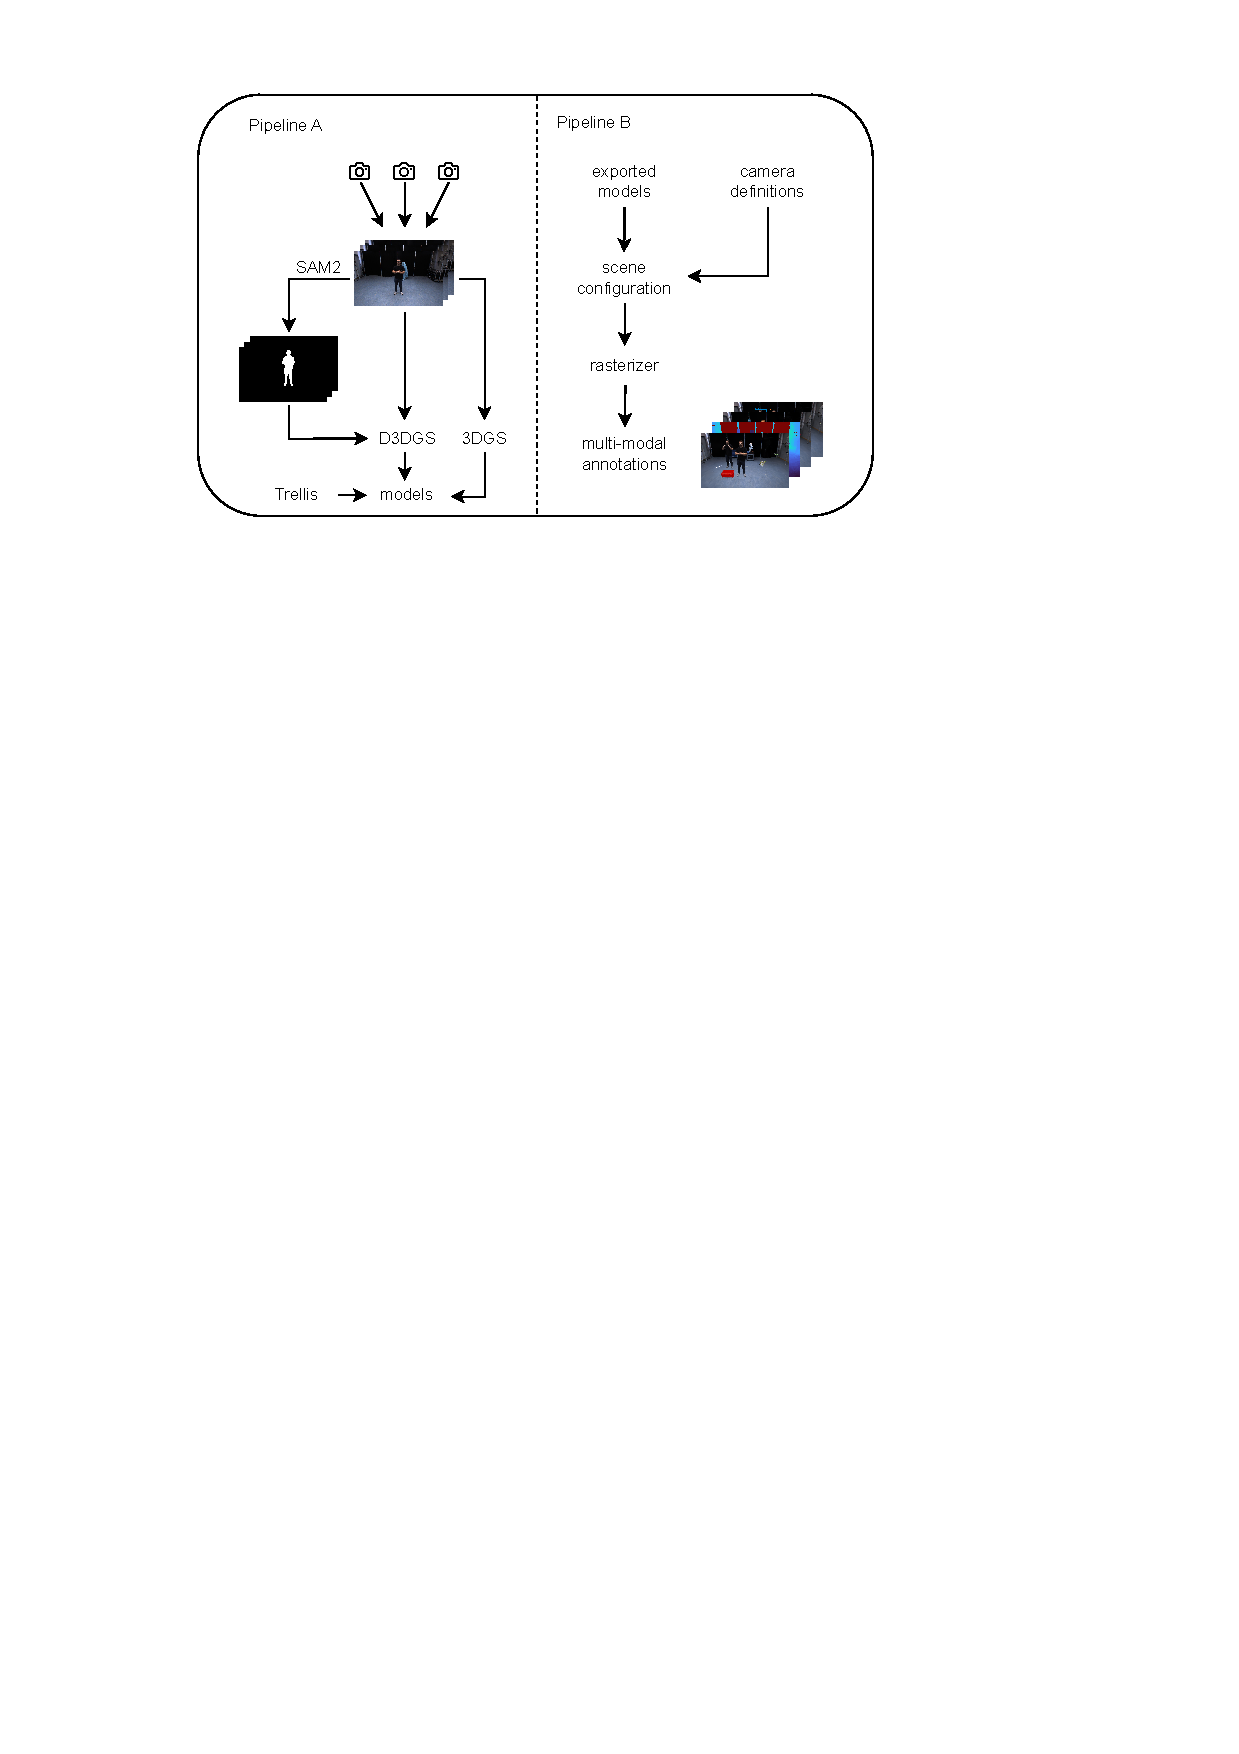
\includegraphics[width=0.9\textwidth]{Grafiken/Ablauf.pdf}
    \caption{
       \textbf{Overview of the proposed composition pipeline.}
        \textbf{Pipeline A} converts multi-view captures into per-object 3DGS and D3DGS models via calibration, mask generation, and model training.
        \textbf{Pipeline B} composes exported models into multi-object scenes, producing synchronized RGB, depth, segmentation, and occlusion annotations.
    }
    \label{fig:Ablauf}
\end{figure*}


\section{Pipeline A: Reconstruction of 3D and Dynamic 3D Models}

The first stage of the system, referred to as \emph{Pipeline A}, transforms synchronized multi-view image sequences into individual Gaussian Splatting models. It uses a high-density capture rig and follows four main stages: capture and calibration, preprocessing, mask generation, and model training.

\subsection{Capture setup and calibration}
The acquisition takes place in a custom-built multi-camera rig equipped with 56 globally synchronized cameras operating at a resolution of \(1920 \times 1200\) pixels and a frame rate of 30 frames per second. 
All cameras are connected to a shared hardware trigger that provides a global clock signal, guaranteeing microsecond-level temporal synchronization across all views.
The cameras are arranged in a hemispherical configuration around a capture volume of approximately \(1.5 \times 1.5 \times 2.5\) meters.
The geometric center of this volume serves as the global origin for all reconstructions.
This setup ensures dense overlapping views and uniform angular coverage, which are essential for complete and consistent 3D and 4D reconstructions.

Calibration is performed in two stages. Intrinsic parameters are estimated for each camera individually following the standard OpenCV pinhole model with five distortion coefficients \((k_1, k_2, p_1, p_2, k_3)\). The intrinsic model comprises focal length, principal point, and both radial and tangential distortion terms.
Because the optical center \((c_x, c_y)\) of each lens is not necessarily aligned with the image center, an \emph{optimal new camera matrix} is computed using OpenCV’s rectification routines to balance field of view and minimal distortion. This step yields undistorted, rectified images that serve as input for all subsequent stages.
Extrinsic calibration is performed once for the entire rig via a global optimization of inter-camera correspondences obtained from a moving checkerboard sequence. 
The resulting extrinsic parameters define all cameras within a unified world coordinate frame.  

\subsection{Data Preparation: Mask Generation and Prompt Propagation}
\label{sec:maskgen}

Dynamic 3D Gaussian Splatting requires per-frame object masks to disentangle dynamic objects from the static background and to maintain temporal consistency during training \cite{luiten2024dynamic}. While the reference implementation primarily relies on binary foreground/background masks, this pipeline extends that step by integrating \textbf{SAM2} \cite{ravi2024sam2}, enabling interactive prompting and high-quality instance segmentation across frames.

Segmentation is initialized by selecting a seed frame and providing manual point or box prompts for the objects of interest. These seed prompts are propagated across all cameras in the calibrated multi-view setup. Concretely, for each camera in the sequence the corresponding seed image is used to generate an initial segmentation prompt that is added to the predictor state, ensuring consistent initial object masks across views. Subsequently, masks are propagated temporally across the sequence using the SAM2 video predictor. This procedure yields temporally consistent, per-camera instance masks for all frames of the dataset. Compared to classical foreground/background segmentation, this approach permits fine-grained object delineation and is more resilient to occlusions and appearance changes across time and viewpoints. The resulting masks are fed directly into the D3DGS training pipeline to supervise dynamic object reconstruction.

\subsection{3D / Dynamic-3D Gaussian Model Training}
\label{sec:modeltraining}

Per-object Gaussian Splatting models are trained using the rectified images, calibrated poses, and instance masks. Static instances are reconstructed with 3DGS~\cite{kerbl3Dgaussians}; dynamic instances use persistent D3DGS~\cite{luiten2024dynamic}. 

The training procedure follows the original methods with two notable deviations. First, Gaussian positions are not initialized from sparse COLMAP point clouds. Because the multi-camera rig is pre-calibrated with known intrinsics and extrinsics, no additional SfM reconstruction is required for each scene. Instead, random point clouds are used to initialize each scene, significantly reducing overhead when training new sequences. Second, all reconstructions share a common global coordinate system, guaranteeing consistent alignment across different captures. Consequently, models trained in separate sequences can be merged directly without additional markers, manual registration, or extra calibration steps.

\paragraph{External 3D assets.}
In addition to models reconstructed with 3DGS and D3DGS, Pipeline A can incorporate externally generated 3D assets. To demonstrate this, small object models produced with \textbf{Trellis}~\cite{xiang2024structured} are used; Trellis reconstructs compact GLB meshes from a few input images and can export models as Gaussian representations. Exported Gaussian assets are imported without modification into the composition framework, demonstrating compatibility with heterogeneous 3D sources such as small household objects (e.g., boxes, plants, or tools).

\section{Pipeline B: Composition and Synthetic Dataset Generation}

While Pipeline A focuses on reconstructing individual static and dynamic Gaussian models, Pipeline B composes these models into coherent multi-object scenes. Pipeline B combines exported models, places them in calibrated virtual environments, and produces synchronized outputs such as RGB images, depth maps, and segmentation masks. The pipeline thus connects reconstruction and dataset generation by providing all necessary modalities for synthetic training and evaluation.

\subsection{Scene configuration and class indexing}
A synthetic scene is defined by a structured list of object instances, each associated with placement parameters and camera trajectories used for rendering. Every object model is assigned a fixed class index that remains consistent throughout the dataset. These indices, together with the scene configuration, are recorded in a JSON manifest that serves as the central reference for all annotations. Each instance also receives a unique identifier and a stable display color from a predefined palette, ensuring consistent instance-level segmentation across frames and scenes. Once configuration is complete, the scene can be rendered either from the physical rig cameras or from virtual viewpoints.

\subsection{Camera definition and interpolation}
The pipeline supports both real and virtual camera configurations. Rendering may be performed using the original rig calibration or via interpolated viewpoints that generate smooth camera paths. Physical camera poses are interpolated while averaging intrinsic parameters to obtain continuous motion through the virtual environment. Temporal supersampling can optionally create intermediate frames through sub-frame interpolation of the Gaussian parameters. This yields smoother apparent motion and higher effective frame rates, which are useful for generating realistic video sequences and temporally consistent annotations.

\subsection{Placement duplication and motion handling}
Objects are positioned in the global coordinate system using rigid transformations composed of translation, rotation, and uniform scaling. Dynamic models carry time-dependent Gaussian attributes and are rendered according to their internal trajectories. The system allows objects to be duplicated and repositioned while maintaining unique instance identifiers. This flexibility enables the creation of diverse scene configurations with varying spatial arrangements and interactions between static and dynamic elements. The same set of reconstructed assets can therefore be reused across many compositions without retraining or manual adjustment.

\subsection{Mask rendering and mask types}
During scene composition, each object is rasterized independently into an object identifier buffer while performing depth testing to ensure correct occlusion ordering. The system exports two complementary mask variants that support different training scenarios. The \emph{visible mask} contains only pixels that remain visible after depth compositing, while the \emph{complete mask} is obtained by rendering the object in isolation and thresholding its depth and alpha values. The complete mask therefore contains the full object silhouette, including regions that may be occluded in the final composition. Providing both mask types ensures compatibility with various downstream pipelines: some models require visible masks for instance segmentation, while others benefit from complete masks for occlusion-aware augmentation.

\paragraph{Occlusion scoring}
For each frame \(t\) and instance \(i\), an occlusion score is computed as
\[
s_{\mathrm{occ}}(t,i) = 1 - \frac{|V_{t,i}|}{|C_{t,i}|},
\]
where \(V_{t,i}\) and \(C_{t,i}\) denote the pixel counts of the visible and complete masks, respectively. The score ranges from 0 (fully visible) to 1 (completely occluded). Occlusion scores are stored in the JSON manifest and can be used for filtering, sampling, or weighting during downstream training.

\subsection{6D pose estimation}
For each object instance, a rigid transformation 
$T_{\mathrm{obj}\rightarrow\mathrm{cam}} \in \mathbb{R}^{4\times4}$ 
is estimated to map canonical object coordinates into the current camera frame. 
The translation component is derived from the displacement of the object centroid, 
computed either over all Gaussian means or a designated subset of anchor points:
\begin{align}
t &= \bar{x}_{t} - \bar{x}_{0}, \\
\bar{x}_{t} &= \frac{1}{|\mathcal{A}|} \sum_{i \in \mathcal{A}} x_i^{(t)}.
\end{align}

Rotational change is obtained from the per-anchor quaternions 
$q_i^{(t)} = (w,x,y,z)$ using Markley’s quaternion averaging method~\cite{markley2007averaging}. 
A mean quaternion is computed for both the reference and current frame:
\begin{align}
q^{(t)}_{\mathrm{mean}} &= 
\arg\max_{\|q\|=1} q^\top
\left(\sum_i q_i^{(t)} q_i^{(t)\top}\right) q,
\end{align}
and the relative rotation is given by
\begin{align}
q_{\Delta} &= q^{(t)}_{\mathrm{mean}} \otimes \overline{q^{(0)}_{\mathrm{mean}}}, \\
R_{\Delta} &= \mathrm{quat2mat}(q_{\Delta}).
\end{align}

The resulting rotation is combined with an optional initial alignment $R_0$, yielding
\begin{align}
R_{\mathrm{obj}} = R_{\Delta} R_0.
\end{align}

Finally, the object-to-camera transform is assembled as
\begin{align}
T_{\mathrm{obj}\rightarrow\mathrm{cam}} =
\left(T_{\mathrm{w}\rightarrow\mathrm{c}}^{-1}\right)
\begin{bmatrix}
R_{\mathrm{obj}} & \bar{x}_{t} \\
0 & 1
\end{bmatrix}.
\end{align}

This transformation represents a temporally consistent 6D pose estimate 
that captures the object’s centroid and orientation changes over time. 
Although these poses are not absolute ground truth, 
they provide reliable internal motion estimates that can be leveraged 
for downstream tasks such as motion tracking, pose refinement, or activity recognition.



\subsection{Keypoint detection and propagation}
The system generates 3D keypoints for each captured dynamic human model. Keypoints for each dynamic human model are initially detected in a reference frame using a Detectron2-based detector \cite{Detectron22020}. The rasterizer was extended to return per-pixel Gaussian indices, enabling tracking of keypoints over time by associating them with the Gaussians that influence the corresponding 2D pixel locations. To ensure temporal consistency across frames, 2D keypoints are reprojected into 3D using rendered depth maps together with camera intrinsics and extrinsics. These 3D points are subsequently updated in each frame according to the motion of the associated 3D Gaussians, ensuring that keypoints follow the dynamic objects throughout the sequence.

\subsection{Rendered outputs and metadata}
For each rendered frame and camera, the pipeline exports RGB images, depth maps, per-instance visible and complete masks, bounding boxes, and object metadata.
All outputs are indexed in a JSON manifest that stores camera parameters, object transformations, occlusion scores, and keypoints, ensuring consistent synchronization across modalities.
For validation and manual inspection the pipeline can additionally output diagnostic overlays such as mask overlays, rendered bounding boxes, and projected 6D poses and keypoints.

\smallskip
Together, these components form a unified, reproducible system for scene composition and dataset generation from modular Gaussian-based models.
